\subsection{Развертывание программного средства}
\label{sec:design:deployment}

После выявления, а также завершения проектирования всех компонентов программного средства появляется вопрос о планировании развертывания всей системы. Необходимо составить описание требуемых аппаратно-программных комплексов, которые понадобятся для обеспечения функционирования распределенного приложения. Для этих целей целесообразным выглядит составление диаграммы развертывания стандарта \uml. 

\begin{figure}[H]
\centering
	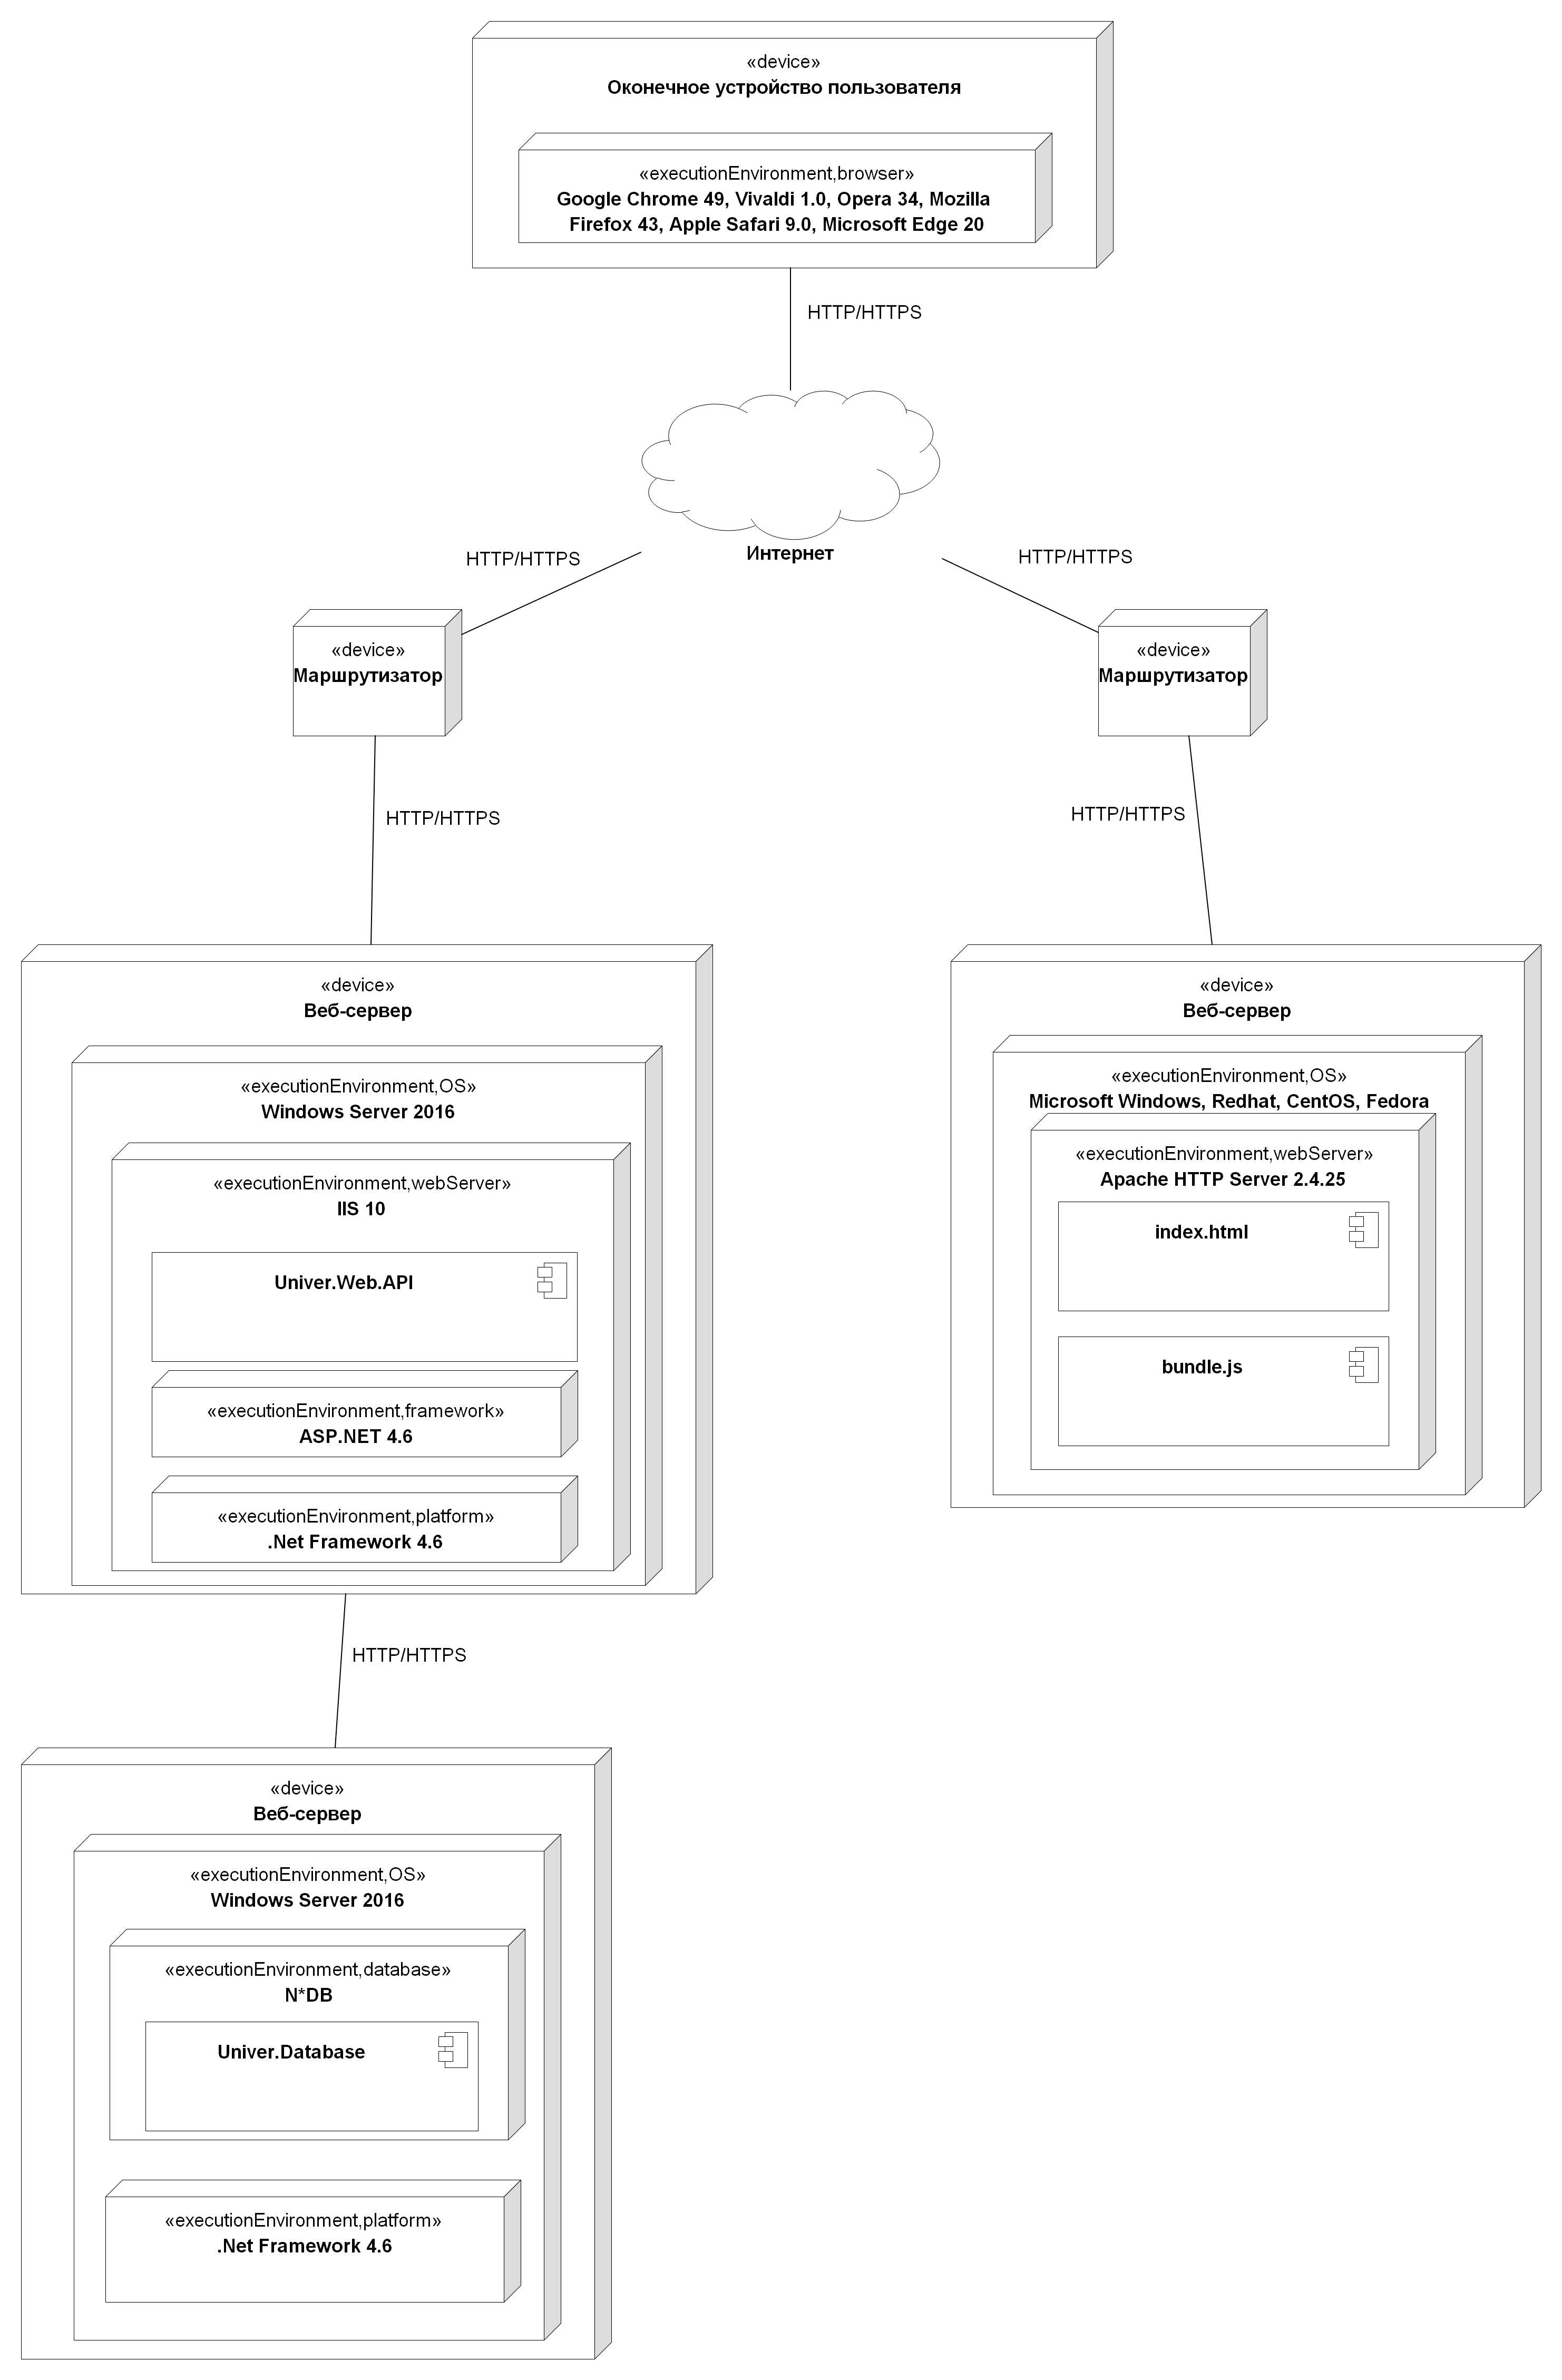
\includegraphics[scale=0.15]{deployment_diagram.png}
	\caption{Диаграмма развертывания ПС}
	\label{fig:design:deployment:diagram}
\end{figure}

Данная диаграмма представлена на рисунке~\ref{fig:design:deployment:diagram}. Она отражает следующие особенности развертывания:

\begin{itemize}
	\item На узле оконечного устройства в качестве среды выполнения перечислен список браузерных программных средств, с помощью которых можно использовать клиентскую часть приложения.
	\item В качестве операционной системы для сервера клиентской части перечислен список поддерживаемых веб-сервером ОС.
	\item При необходимости Apache HTTP Server может быть заменен другим HTTP-сервером.
	\item Для серверной части программного средства и базы данных показано их развертывание на отдельных узлах. При самом развертывании в зависимости от условий поставщика вычислительных мощностей данные элементы программной системы могут быть объединены на одном узле.
	\item В свою очередь, помимо упрощения, возможно и усложнение схемы развертывания, например, база данных будет развернута на нескольких узлах. Тем не менее, все узлы должны удовлетворять отображенным условиям.
	\item Все серверы: и клиентской части, и серверной, и базы данных, -- могут быть физически расположены в различных дата-центрах.
	\item Предполагается, что пользовательское оконечное устройство зна\-чи\-те\-льно удалено от серверов программной системы, доступ осуществляется через сеть Интернет, что и упрощенно показано на диаграмме.
\end{itemize}

Таким образом, после развертывания программного средства пользователи могут уже начать им пользоваться.
